\documentclass[a4paper,12pt]{article}
\usepackage{amsmath, amssymb, amsfonts, bm}
\usepackage{geometry}
\usepackage{tcolorbox}
\usepackage{tikz}
\usepackage{tikz-cd}
\usepackage{mathtools}
\usepackage{caption}
\usepackage{thmtools}
\usepackage{hyperref}
\usepackage{float}
\geometry{margin=2.5cm}

\declaretheorem[style=definition, name=Theorem, numberwithin=section]{theorem}
\declaretheorem[style=definition, name=Proof, sibling=theorem]{proof}
\declaretheorem[style=definition, name=Proposition, sibling=theorem]{proposition}
\declaretheorem[style=definition, name=Corollary, sibling=theorem]{corollary}

\title{Parametric Sensitivity in Optimization\\
\large A Comprehensive Treatment with Theoretical Foundations}
\author{}
\date{}

% Box styles
\tcbset{
    myformula/.style={colback=blue!5!white, colframe=blue!75!black, sharp corners, boxrule=0.8pt, left=2mm, right=2mm, top=1mm, bottom=1mm},
    myexample/.style={colback=green!5!white, colframe=green!75!black, sharp corners, boxrule=0.8pt, left=2mm, right=2mm, top=1mm, bottom=1mm},
    mynote/.style={colback=yellow!5!white, colframe=yellow!75!black, sharp corners, boxrule=0.8pt, left=2mm, right=2mm, top=1mm, bottom=1mm},
    mytheorem/.style={colback=red!5!white, colframe=red!75!black, sharp corners, boxrule=1pt, left=3mm, right=3mm, top=2mm, bottom=2mm}
}

\begin{document}

\maketitle

\section{Introduction and Problem Setup}

Consider a parametric optimization problem:
\[
P(p): \quad \min_{x \in \mathbb{R}^n} f(x,p), \quad p \in \mathbb{R}^m
\]
where $f: \mathbb{R}^n \times \mathbb{R}^m \to \mathbb{R}$ is twice continuously differentiable, and $x^*(p)$ denotes the optimal solution (or a local minimizer) for parameter $p$.

\begin{tcolorbox}[title=Historical Context, mynote]
The study of parametric optimization dates back to the work of \textit{Fiacco and McCormick} (1968) on nonlinear programming. The fundamental theoretical foundation is provided by the \textit{Implicit Function Theorem} applied to optimality conditions.
\end{tcolorbox}

\textbf{Goal:} Understand the mapping $p \mapsto x^*(p)$ and compute its derivative $\frac{\partial x^*}{\partial p}$, known as the \textit{sensitivity matrix} or \textit{parametric gradient}.

\section{Theoretical Foundations}

\subsection{Implicit Function Theorem Approach}

Let $\nabla_x f(x,p)$ denote the gradient of $f$ with respect to $x$. For unconstrained problems, the first-order necessary condition is:

\begin{theorem}[Implicit Function Theorem for Optimization]
Assume $f(x,p)$ is $C^2$ in a neighborhood of $(x_0, p_0)$, and $\nabla_x f(x_0, p_0) = 0$. If the Hessian $\nabla^2_{xx} f(x_0, p_0)$ is nonsingular, then there exists a neighborhood $U$ of $p_0$ and a unique $C^1$ function $x^*: U \to \mathbb{R}^n$ such that:
\begin{enumerate}
    \item $x^*(p_0) = x_0$
    \item $\nabla_x f(x^*(p), p) = 0$ for all $p \in U$
    \item $\frac{\partial x^*}{\partial p}(p_0) = -[\nabla^2_{xx} f(x_0, p_0)]^{-1} \nabla^2_{xp} f(x_0, p_0)$
\end{enumerate}
\end{theorem}

\begin{proof}
The result follows directly from the classical Implicit Function Theorem applied to the equation $\nabla_x f(x,p) = 0$. Differentiating this identity with respect to $p$ gives:
\[
\nabla^2_{xx} f(x^*(p), p) \frac{\partial x^*}{\partial p} + \nabla^2_{xp} f(x^*(p), p) = 0
\]
Solving for $\frac{\partial x^*}{\partial p}$ yields the sensitivity formula.
\end{proof}

\section{Unconstrained Optimization: Sensitivity Analysis}

\subsection{Basic Sensitivity Formula}

Applying Theorem 2.1 directly, we obtain:

\begin{tcolorbox}[title=Sensitivity Formula (Unconstrained), myformula]
\[
S(p) \triangleq \frac{\partial x^*}{\partial p}(p) = - [\nabla^2_{xx} f(x^*(p), p)]^{-1} \cdot \nabla^2_{xp} f(x^*(p), p)
\]
\end{tcolorbox}

\subsection{Geometric Interpretation}

The sensitivity matrix $S(p) \in \mathbb{R}^{n \times m}$ has important interpretations:

\begin{figure}[H]
\centering
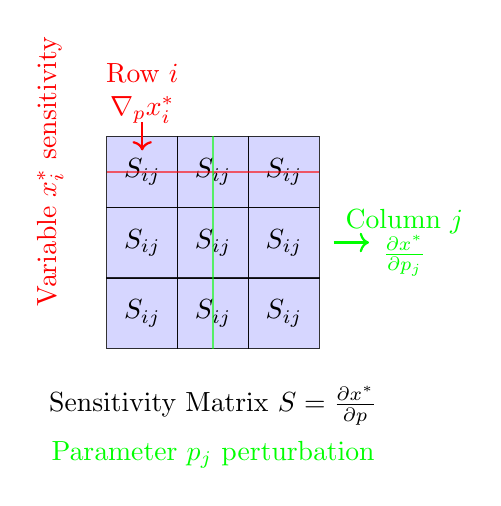
\begin{tikzpicture}[scale=0.9]
% Matrix cells
\foreach \i in {0,1,2} {
    \foreach \j in {0,1,2} {
        \draw[fill=blue!20, opacity=0.8] (\j,\i) rectangle (\j+1,\i+1);
        \node at (\j+0.5, \i+0.5) {$S_{ij}$};
    }
}

% Labels
\node at (1.5, -0.8) {Sensitivity Matrix $S = \frac{\partial x^*}{\partial p}$};

% Row interpretation
\draw[->, thick, red] (0.5,3.2) -- (0.5,2.8);
\node[red, align=center] at (0.5,3.6) {Row $i$\\ $\nabla_p x_i^*$};
\draw[red, thick, opacity=0.6] (0,2.5) -- (3,2.5);
\node[red, rotate=90] at (-0.8,2.5) {Variable $x_i^*$ sensitivity};

% Column interpretation  
\draw[->, thick, green] (3.2,1.5) -- (3.7,1.5);
\node[green, align=center] at (4.2,1.5) {Column $j$\\ $\frac{\partial x^*}{\partial p_j}$};
\draw[green, thick, opacity=0.6] (1.5,0) -- (1.5,3);
\node[green] at (1.5, -1.5) {Parameter $p_j$ perturbation};
\end{tikzpicture}
\caption{Geometric interpretation of the sensitivity matrix. Rows represent gradients of individual variables with respect to all parameters. Columns represent how the entire solution vector responds to individual parameters.}
\label{fig:matrix_interpretation}
\end{figure}

\textbf{Interpretations:}
\begin{itemize}
    \item \textbf{Row $i$:} Gradient of $x_i^*$ with respect to $p \in \mathbb{R}^m$
    \item \textbf{Column $j$:} Response of entire solution $x^*$ to parameter $p_j$
    \item \textbf{Entry $S_{ij}$:} $\frac{\partial x_i^*}{\partial p_j}$, local linear approximation of how variable $i$ changes with parameter $j$
\end{itemize}

\subsection{Example and Verification}

\begin{tcolorbox}[title=Quadratic Example, myexample]
Consider $f(x,a,b) = \frac{1}{2}ax^2 + bx$, with $a>0$. The solution is $x^*(a,b) = -\frac{b}{a}$.

\textbf{Direct computation:}
\[
\frac{\partial x^*}{\partial a} = \frac{b}{a^2}, \quad \frac{\partial x^*}{\partial b} = -\frac{1}{a}
\]

\textbf{Sensitivity formula:}
\[
\nabla^2_{xx} f = a, \quad \nabla^2_{xa} f = x, \quad \nabla^2_{xb} f = 1
\]
At optimum $x^* = -b/a$:
\[
\frac{\partial x^*}{\partial a} = -a^{-1} \cdot x^* = -a^{-1}(-b/a) = b/a^2
\]
\[
\frac{\partial x^*}{\partial b} = -a^{-1} \cdot 1 = -1/a
\]
The results match perfectly.
\end{tcolorbox}

\section{Constrained Optimization: Box Constraints}

\subsection{KKT Conditions and Active Sets}

For the box-constrained problem:
\[
\min_{l \leq x \leq u} f(x,p)
\]
the KKT conditions are:
\[
\nabla_x f(x^*,p) + \lambda^+ - \lambda^- = 0
\]
with complementarity conditions:
\[
\lambda_i^+ \geq 0, \quad \lambda_i^- \geq 0, \quad \lambda_i^+(x_i^* - u_i) = 0, \quad \lambda_i^-(l_i - x_i^*) = 0
\]

We define the \textit{active} and \textit{free} sets:
\begin{align*}
A_L(p) &= \{i: x_i^*(p) = l_i\} \quad \text{(lower bound active)}\\
A_U(p) &= \{i: x_i^*(p) = u_i\} \quad \text{(upper bound active)}\\
F(p) &= \{i: l_i < x_i^*(p) < u_i\} \quad \text{(free variables)}
\end{align*}

\begin{figure}[H]
\centering
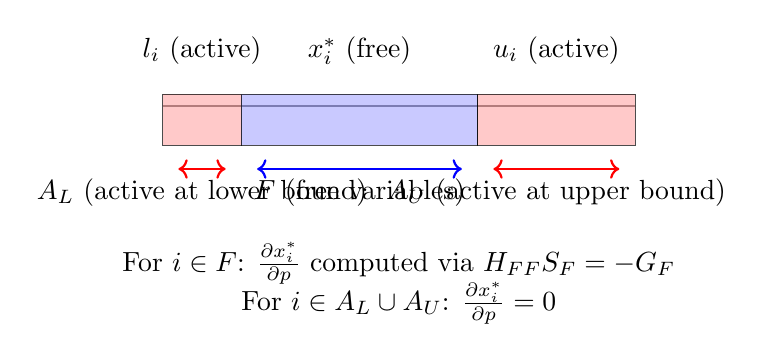
\begin{tikzpicture}[scale=1]
% Main line
\draw[thick] (0,0) -- (6,0);

% Active and free regions
\draw[fill=red!30, opacity=0.7] (0,-0.5) rectangle (1,0.15);  
\node at (0.5,0.7) {$l_i$ (active)};
\draw[fill=blue!30, opacity=0.7] (1,-0.5) rectangle (4,0.15); 
\node at (2.5,0.7) {$x_i^*$ (free)};
\draw[fill=red!30, opacity=0.7] (4,-0.5) rectangle (6,0.15);  
\node at (5,0.7) {$u_i$ (active)};

% Labels with arrows
\draw[<->, thick, red] (0.2,-0.8) -- (0.8,-0.8);
\node at (0.5,-1.1) {$A_L$ (active at lower bound)};

\draw[<->, thick, blue] (1.2,-0.8) -- (3.8,-0.8);
\node at (2.5,-1.1) {$F$ (free variables)};

\draw[<->, thick, red] (4.2,-0.8) -- (5.8,-0.8);
\node at (5,-1.1) {$A_U$ (active at upper bound)};

% Additional annotations
\node[align=center] at (3,-2) {For $i \in F$: $\frac{\partial x_i^*}{\partial p}$ computed via $H_{FF}S_F = -G_F$};
\node[align=center] at (3,-2.5) {For $i \in A_L \cup A_U$: $\frac{\partial x_i^*}{\partial p} = 0$};
\end{tikzpicture}
\caption{Active and free sets in box-constrained optimization. Free variables have sensitivities computed from the reduced Hessian, while active variables have zero sensitivity as long as the active set remains unchanged.}
\label{fig:active_free_sets}
\end{figure}

\subsection{Sensitivity with Fixed Active Set}

\begin{theorem}[Sensitivity with Box Constraints]
Assume the \textit{strict complementarity} condition holds: for active bounds, the corresponding Lagrange multipliers are positive. If the active set remains constant in a neighborhood of $p_0$, then:
\begin{enumerate}
    \item For $i \in F$: $\frac{\partial x_i^*}{\partial p}$ satisfies $H_{FF} \frac{\partial x_F^*}{\partial p} = -G_F$
    \item For $i \in A_L \cup A_U$: $\frac{\partial x_i^*}{\partial p} = 0$
\end{enumerate}
where $H_{FF} = \nabla^2_{x_F x_F} f$ and $G_F = \nabla^2_{x_F p} f$.
\end{theorem}

\begin{proof}
For free variables, the constraints are inactive, so the sensitivity follows from the unconstrained case restricted to $F$. For active variables, $x_i^*$ is fixed at the bound, so its derivative with respect to $p$ is zero as long as the active set doesn't change.
\end{proof}

\subsection{Active Set Changes and Nondifferentiability}

\begin{tcolorbox}[title=Critical Warning: Nondifferentiability, mynote]
The mapping $p \mapsto x^*(p)$ is generally \textbf{not differentiable} at points where the active set changes. This occurs when:
\begin{itemize}
    \item A free variable hits a bound
    \item An active variable leaves a bound
\end{itemize}
At such points, the sensitivity may be discontinuous or undefined.
\end{tcolorbox}

\subsection{Flowchart: Active Set Management}

\begin{figure}[H]
\centering
\begin{tikzcd}[row sep=2em, column sep=3em, ampersand replacement=\&]
p \text{ changes} \arrow[r] \& 
\text{Solve KKT conditions} \arrow[r, "{\text{Check activity}}"] \& 
\text{Active set constant?} \arrow[d, "{\text{Yes}}"'] \arrow[dd, "{\text{No}}"] \\
\& \& 
\text{Compute } S_F = -H_{FF}^{-1} G_F \arrow[d] \\
\& \& 
\text{Update sensitivity } S \\
\& \& 
\text{Re-identify } F, A_L, A_U \arrow[u]
\end{tikzcd}
\caption{Flowchart for managing active set changes in sensitivity computation. When the active set changes, sensitivity becomes nondifferentiable and must be recomputed with the new active set.}
\label{fig:active_set_flowchart}
\end{figure}

\section{L2-Regularized Problem with Center}

\subsection{Centered Regularization Formulation}

We consider the regularized problem with a center point $x_0$:
\[
\min_{x \in \mathbb{R}^n} f(x,p) + \frac{\varepsilon}{2} \|x - x_0\|^2
\]
where $\varepsilon > 0$ is the regularization parameter and $x_0 \in \mathbb{R}^n$ is a fixed reference point.

\begin{proposition}[Regularized Optimality Condition]
The optimal solution $x^*_\varepsilon(p)$ satisfies:
\[
\nabla_x f(x^*_\varepsilon(p), p) + \varepsilon (x^*_\varepsilon(p) - x_0) = 0
\]
\end{proposition}

\begin{theorem}[Sensitivity for Centered Regularization]
The sensitivity of the regularized solution is given by:
\[
\frac{\partial x^*_\varepsilon}{\partial p}(p) = - [\nabla^2_{xx} f(x^*_\varepsilon(p), p) + \varepsilon I]^{-1} \cdot \nabla^2_{xp} f(x^*_\varepsilon(p), p)
\]
\end{theorem}

\begin{proof}
Differentiate the regularized optimality condition with respect to $p$:
\[
[\nabla^2_{xx} f + \varepsilon I] \frac{\partial x^*_\varepsilon}{\partial p} + \nabla^2_{xp} f = 0
\]
Note that $\frac{\partial x_0}{\partial p} = 0$ since $x_0$ is fixed. Solving for $\frac{\partial x^*_\varepsilon}{\partial p}$ gives the result.
\end{proof}

\subsection{Properties and Interpretation}

\begin{corollary}[Regularization Effects]
The centered L2-regularization has several beneficial effects:
\begin{enumerate}
    \item \textbf{Improved conditioning:} $\kappa(H + \varepsilon I) \leq \kappa(H)$ for $\varepsilon > 0$
    \item \textbf{Bounded sensitivity:} $\|S_\varepsilon\| \leq \frac{\|G\|}{\varepsilon}$ when $H \succeq 0$
    \item \textbf{Bias-variance tradeoff:} $x^*_\varepsilon$ is biased toward $x_0$ but has lower variance
\end{enumerate}
\end{corollary}

\begin{tcolorbox}[title=Bayesian Interpretation, myexample]
The centered regularization term $\frac{\varepsilon}{2}\|x-x_0\|^2$ corresponds to a Gaussian prior $x \sim \mathcal{N}(x_0, \varepsilon^{-1}I)$ in Bayesian inference. The sensitivity formula then gives the posterior covariance structure.
\end{tcolorbox}

\section{Visualization of Matrix Relationships}

\begin{figure}[H]
\centering
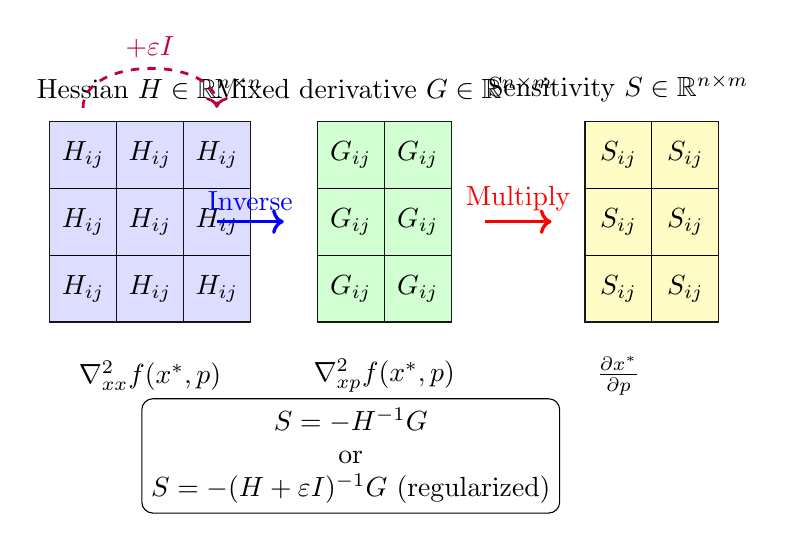
\begin{tikzpicture}[scale=0.85]
% Hessian matrix (n x n)
\foreach \i in {0,1,2} {
    \foreach \j in {0,1,2} {
        \draw[fill=blue!15, opacity=0.9] (\j,\i) rectangle (\j+1,\i+1);
        \node at (\j+0.5, \i+0.5) {$H_{ij}$};
    }
}
\node at (1.5, 3.5) {Hessian $H \in \mathbb{R}^{n\times n}$};
\node at (1.5, -0.8) {$\nabla^2_{xx} f(x^*,p)$};

% Mixed derivative matrix (n x m)
\foreach \i in {0,1,2} {
    \foreach \j in {0,1} {
        \draw[fill=green!20, opacity=0.9] (4+\j,\i) rectangle (5+\j,\i+1);
        \node at (4+\j+0.5, \i+0.5) {$G_{ij}$};
    }
}
\node at (5, 3.5) {Mixed derivative $G \in \mathbb{R}^{n\times m}$};
\node at (5, -0.8) {$\nabla^2_{xp} f(x^*,p)$};

% Sensitivity matrix (n x m)
\foreach \i in {0,1,2} {
    \foreach \j in {0,1} {
        \draw[fill=yellow!25, opacity=0.9] (8+\j,\i) rectangle (9+\j,\i+1);
        \node at (8+\j+0.5, \i+0.5) {$S_{ij}$};
    }
}
\node at (8.5, 3.5) {Sensitivity $S \in \mathbb{R}^{n\times m}$};
\node at (8.5, -0.8) {$\frac{\partial x^*}{\partial p}$};

% Arrows showing relationships
\draw[->, thick, blue, line width=1.2pt] (2.5,1.5) to[out=0, in=180] node[midway, above] {Inverse} (3.5,1.5);

\draw[->, thick, red, line width=1.2pt] (6.5,1.5) to[out=0, in=180] node[midway, above] {Multiply} (7.5,1.5);

% Regularization addition
\draw[->, thick, purple, dashed, line width=1pt] (0.5,3.2) to[out=90, in=90] node[midway, above] {$+\varepsilon I$} (2.5,3.2);

% Equation annotation
\node[align=center, draw, rounded corners, fill=white] at (4.5, -2) 
{$S = -H^{-1}G$\\or\\$S = -(H + \varepsilon I)^{-1}G$ (regularized)};
\end{tikzpicture}
\caption{Visual representation of matrix relationships in sensitivity computation. The Hessian matrix $H$ (blue) is inverted and multiplied by the mixed derivative matrix $G$ (green) to obtain the sensitivity matrix $S$ (yellow). The purple dashed arrow indicates regularization by adding $\varepsilon I$ to the Hessian.}
\label{fig:matrix_relationships}
\end{figure}

\section{Algorithmic Implementation}

\subsection{Pseudocode for Sensitivity Computation}

\begin{tcolorbox}[title=Algorithm: Parametric Sensitivity Computation, myformula]
\begin{enumerate}
    \item \textbf{Input:} $p_0$ (parameter), $\varepsilon$ (regularization, optional), $x_0$ (center, optional)
    \item \textbf{Solve:} $x^* \leftarrow \arg\min_x f(x,p_0) + \frac{\varepsilon}{2}\|x-x_0\|^2$ (with constraints if needed)
    \item \textbf{Compute derivatives:}
    \begin{itemize}
        \item $H \leftarrow \nabla^2_{xx} f(x^*, p_0)$
        \item $G \leftarrow \nabla^2_{xp} f(x^*, p_0)$
    \end{itemize}
    \item \textbf{If regularized:} $H \leftarrow H + \varepsilon I$
    \item \textbf{If constrained:}
    \begin{itemize}
        \item Identify active set $A$ and free set $F$
        \item Extract $H_{FF}$, $G_F$
        \item Solve $H_{FF} S_F = -G_F$
        \item Set $S_A = 0$
    \end{itemize}
    \item \textbf{Else:} Solve $H S = -G$
    \item \textbf{Output:} $x^*$, $S = \frac{\partial x^*}{\partial p}$
\end{enumerate}
\end{tcolorbox}

\subsection{Computational Considerations}

\begin{itemize}
    \item \textbf{Matrix inversion:} Use Cholesky or LU decomposition for $H$ or $H_{FF}$
    \item \textbf{Sparsity:} Exploit sparsity in $H$ and $G$ for large-scale problems
    \item \textbf{Adjoint method:} For many parameters ($m \gg n$), compute $S^T = -G^T H^{-1}$ more efficiently
    \item \textbf{Warm-starting:} Use $x^*(p_0) + S \Delta p$ as initial guess for $x^*(p_0 + \Delta p)$
\end{itemize}

\section{Applications and Extensions}

\subsection{Practical Applications}

\begin{itemize}
    \item \textbf{Optimal Control:} Sensitivity of optimal trajectories to model parameters
    \item \textbf{Model Predictive Control (MPC):} Fast gradient computation for real-time optimization
    \item \textbf{Machine Learning:} Hyperparameter tuning via gradient-based methods
    \item \textbf{Design Optimization:} Sensitivity of optimal designs to requirements
    \item \textbf{Economics:} Comparative statics in economic equilibrium models
\end{itemize}

\subsection{Extensions in Literature}

\begin{tcolorbox}[title=Advanced Topics, mynote]
\begin{itemize}
    \item \textbf{Second-order sensitivity:} $\frac{\partial^2 x^*}{\partial p^2}$ via tensor methods
    \item \textbf{Non-smooth problems:} Generalized derivatives and Clarke calculus
    \item \textbf{Stochastic parameters:} Sensitivity in expectation $\mathbb{E}[x^*(p)]$
    \item \textbf{Bilevel optimization:} Sensitivity of upper-level to lower-level solutions
    \item \textbf{Sensitivity of KKT multipliers:} $\frac{\partial \lambda^*}{\partial p}$ for active constraints
\end{itemize}
\end{tcolorbox}

\section{Historical Notes and References}

\subsection{Foundational Works}

\begin{enumerate}
    \item \textbf{Fiacco, A.V. \& McCormick, G.P.} (1968). \textit{Nonlinear Programming: Sequential Unconstrained Minimization Techniques}. Wiley.
    \item \textbf{Fiacco, A.V.} (1983). \textit{Introduction to Sensitivity and Stability Analysis in Nonlinear Programming}. Academic Press.
    \item \textbf{Bonnans, J.F. \& Shapiro, A.} (2000). \textit{Perturbation Analysis of Optimization Problems}. Springer.
    \item \textbf{Dontchev, A.L. \& Rockafellar, R.T.} (2014). \textit{Implicit Functions and Solution Mappings: A View from Variational Analysis}. Springer.
\end{enumerate}

\subsection{Modern Developments}

\begin{enumerate}
    \item \textbf{Amos, B. \& Kolter, J.Z.} (2017). OptNet: Differentiable optimization as a layer in neural networks. \textit{ICML}.
    \item \textbf{Gould, S., Fernando, B., Cherian, A., \textit{et al.}} (2016). On differentiating parameterized argmin and argmax problems with application to bi-level optimization. \textit{arXiv:1607.05447}.
    \item \textbf{Blondel, M., Berthet, Q., Cuturi, M., \textit{et al.}} (2022). Efficient and modular implicit differentiation. \textit{Advances in Neural Information Processing Systems}.
\end{enumerate}

\section*{Conclusion}

Parametric sensitivity analysis provides powerful tools for understanding how optimal solutions respond to parameter changes. The centered regularization approach offers numerical stability and Bayesian interpretability while maintaining the same computational structure as standard sensitivity analysis. The theoretical foundations in implicit function theory and KKT conditions provide rigorous guarantees for local sensitivity computations.

\end{document}
